%  LaTeX support: latex@mdpi.com 
%  For support, please attach all files needed for compiling as well as the log file, and specify your operating system, LaTeX version, and LaTeX editor.

%=================================================================
\documentclass[sensors,article,submit,oneauthor]{Definitions/mdpi} 
% For posting an early version of this manuscript as a preprint, you may use "preprints" as the journal. Changing "submit" to "accept" before posting will remove line numbers.

% Below journals will use APA reference format:
% admsci, aieduc, behavsci, businesses, econometrics, economies, education, ejihpe, famsci, games, humans, ijcs, ijfs, investment, fclam, jintelligence, journalmedia, jrfm, jsam, languages, opermanag, peacestud, pmh, psycholint, publications, tourismhosp, youth

% Below journals will use Chicago reference format:
% arts, genealogy, histories, humanities, laws, literature, religions, risks, socsci

%--------------------
% Class Options:
%--------------------
%----------
% journal
%----------
% Choose between the following MDPI journals:
% accountaudit, acn, acoustics, actuators, addictions, addictprev, adhesives, adolescents, aerobiology, aerospace, agriculture, agriengineering, agrochemicals, agronomy, ai, aichem, aieng, aimater, aimed, aipa, air, aisens, aisoc, algorithms, allergies, alloys, amh, analog, analytica, analytics, anatomia, anesthres, animals, antibiotics, antibodies, antioxidants, applbiosci, appliedchem, appliedmath, appliedphys, applmech, applmicrobiol, applnano, applsci, aps, aquacj, archaeolstud, architecture, arm, arthropoda, asc, asi, astronautics, astronomy, atmosphere, atoms, audiolres, automation, axioms, bacteria, batteries, bdcc, beverages, biochem, bioengineering, biologics, biology, biomass, biomechanics, biomed, biomedicines, biomedinformatics, biomimetics, biomolecules, biophysica, bioresourbioprod, biosensors, biosphere, biotech, birds, blockchains, bloods, blsf, brainsci, breath, buildings, cancers, carbon, cardio, cardiogenetics, cardiovascmed, catalysts, cells, ceramics, challenges, chemengineering, chemistry, chemosensors, chemproc, children, chips, cimb, civileng, cleantechnol, climate, clinbioenerg, clinpract, clockssleep, cmd, cmtr, coasts, coatings, colloids, colorants, commodities, complexities, complications, compounds, computation, computers, condensedmatter, conservation, constrmater, cosmetics, covid, crops, cryo, cryptography, crystals, csmf, ctn, culture, curroncol, cyber, dairy, data, ddc, dentistry, dermato, dermatopathology, designs, devices, dhi, diabetology, diagnostics, dietetics, digital, disabilities, diseases, diversity, dna, drones, drugreact, drylands, dynamics, earth, ebj, ecm, ecologies, edm, eesp, electricity, electrochem, electronicmat, electronics, embodiedintell, encyclopedia, endocrines, energies, eng, engproc, entomology, entropy, environments, environremediat, epidemiologia, epigenomes, esa, est, fermentation, fibers, fintech, fire, fishes, fluids, foodeng, foods, forecasting, forensicsci, forests, fossstud, foundations, fractalfract, freshwater, fuels, future, futureinternet, futurepharmacol, futurephys, futuretransp, galaxies, gases, gastroent, gastrointestdisord, gastronomy, gels, genes, geochem, geographies, geohazards, geomatics, geometry, geosciences, geotechnics, geriatrics, germs, glacies, grainsci, grasses, green, greenhealth, gucdd, gynecolcancer, hardware, hazardousmatters, healthcare, healthcmater, hearts, hemato, hematolrep, hep, heritage, higheredu, highthroughput, horticulturae, hospitals, hydrobiology, hydrogen, hydrology, hydrometeorology, hydropower, hygiene, idr, iic, ijem, ijerph, ijgi, ijmd, ijms, ijns, ijom, ijp, ijpb, ijt, ijtm, ijtpp, ijtst, ime, immuno, industries, inflammj, informatics, information, infrastructures, inorganics, insects, instruments, inventions, iot, j, jaestheticmed, jal, japma, jcdd, jcm, jcp, jcrm, jcs, jcto, jdad, jdb, jdream, jemr, jeta, jfb, jfmk, jfth, jgbg, jgg, jimaging, jlpea, jmahp, jmmp, jmms, jmp, jmse, jne, jnt, jof, joi, joitmc, joma, jop, joptm, jor, jox, jpbi, jphytomed, jpm, jsan, jtaer, jvd, jzbg, kidneydial, kinasesphosphatases, knowledge, labmed, laboratories, lam, land, lasers, legumes, life, lights, limnolrev, lipidology, liquids, livers, logics, logistics, lubricants, lymphatics, machines, macromol, magnetism, magnetochemistry, make, marinedrugs, maritime, materials, materproc, mathematics, mca, mcb, measurements, medicina, medicines, medsci, membranes, merits, metabolites, metals, meteorology, methane, metrics, metrology, micro, microarrays, microbiolres, microelectronics, micromachines, microorganisms, microplastics, microwave, minerals, mining, mmphys, modelling, molbank, molecules, mollusca, mps, msf, mti, multimedia, muscles, nanoenergyadv, nanomanufacturing, nanomaterials, ncrna, ndt, network, neuroglia, neuroimaging, neurolint, neurosci, nitrogen, notspecified, nursrep, nutraceuticals, nutrients, obesities, occuphealth, oceans, ohbm, onco, optics, oral, organics, organoids, osteology, oxygen, pandemics, parasites, parasitologia, particles, pathogens, pathophysiology, pediatrrep, pets, pharmaceuticals, pharmaceutics, pharmacoepidemiology, pharmacy, phc, philosophies, photochem, photonics, photovoltaics, phycology, physchem, physics, physiologia, plants, plasma, platforms, pollutants, polymers, polysaccharides, populations, poultry, powders, precision, precisoncol, preprints, proceedings, processes, prosthesis, proteomes, psf, psychiatryint, psychoactives, purification, quantumrep, quaternary, qubs, radiation, rareearths, rdt, reactions, realestate, receptors, recycling, regeneration, remotesensing, reports, reprodmed, resources, rheumato, rjpm, robotics, rsee, ruminants, safety, sanpp, sca, sci, scipharm, sclerosis, seeds, sensors, separations, sexes, shi, signals, sinusitis, siuj, skins, smartcities, smartfish, sna, societies, software, soilsystems, solar, solids, spectroscj, sports, standards, stats, std, stratsediment, stresses, strokerep, superintelligence, surfaces, surgeries, suschem, sustainability, sustainfoods, sustainpackag, symmetry, synbio, systems, tae, targets, taxonomy, technologies, telecom, test, textiles, thalassrep, therapeutics, thermo, timespace, tomography, toxics, toxins, tph, transplantology, transportation, traumacare, traumas, tri, tropicalmed, universe, urbansci, uro, vaccines, vehicles, venereology, vetsci, vibration, virtualworlds, viruses, vision, waste, water, welding, wem, wevj, wild, wind, women, world, zoonoticdis

%---------
% article
%---------
% The default type of manuscript is "article", but can be replaced by: 
% abstract, addendum, article, benchmark, book, bookreview, briefcommunication, briefreport, casereport, changes, clinicopathologicalchallenge, comment, commentary, communication, conceptpaper, conferenceproceedings, correction, conferencereport, creative, datadescriptor, discussion, entry, expressionofconcern, extendedabstract, editorial, essay, erratum, fieldguide, hypothesis, interestingimages, letter, meetingreport, monograph, newbookreceived, obituary, opinion, proceedingpaper, projectreport, reply, retraction, review, perspective, protocol, shortnote, studyprotocol, supfile, systematicreview, technicalnote, viewpoint, guidelines, registeredreport, tutorial,  giantsinurology, urologyaroundtheworld
% supfile = supplementary materials

%----------
% submit
%----------
% The class option "submit" will be changed to "accept" by the Editorial Office when the paper is accepted. This will only make changes to the frontpage (e.g., the logo of the journal will get visible), the headings, and the copyright information. Also, line numbering will be removed. Journal info and pagination for accepted papers will also be assigned by the Editorial Office.

%------------------
% moreauthors
%------------------
% If there is only one author the class option oneauthor should be used. Otherwise use the class option moreauthors.

%=================================================================
% MDPI internal commands - do not modify
\firstpage{1} 
\makeatletter 
\setcounter{page}{\@firstpage} 
\makeatother
\pubvolume{1}
\issuenum{1}
\articlenumber{0}
\pubyear{2026}
\copyrightyear{2026}
%\externaleditor{Firstname Lastname} % More than 1 editor, please add `` and '' before the last editor name
\datereceived{ } 
\daterevised{ } % Comment out if no revised date
\dateaccepted{ } 
\datepublished{ } 
%\datecorrected{} % For corrected papers: "Corrected: XXX" date in the original paper.
%\dateretracted{} % For retracted papers: "Retracted: XXX" date in the original paper.
%\doinum{} % Used for some special journals, like molbank
%\pdfoutput=1 % Uncommented for upload to arXiv.org
%\CorrStatement{yes}  % For updates
%\longauthorlist{yes} % For many authors that exceed the left citation part
%\IsAssociation{yes} % For association journals

%=================================================================
% Add packages and commands here. The following packages are loaded in our class file: fontenc, inputenc, calc, indentfirst, fancyhdr, graphicx, epstopdf, lastpage, ifthen, float, amsmath, amssymb, lineno, setspace, enumitem, mathpazo, booktabs, titlesec, etoolbox, tabto, xcolor, colortbl, soul, multirow, microtype, tikz, totcount, changepage, attrib, upgreek, array, tabularx, pbox, ragged2e, tocloft, marginnote, marginfix, enotez, amsthm, natbib, hyperref, cleveref, scrextend, url, geometry, newfloat, caption, draftwatermark, seqsplit
% cleveref: load \crefname definitions after \begin{document}

%=================================================================
% Please use the following mathematics environments: Theorem, Lemma, Corollary, Proposition, Characterization, Property, Problem, Example, ExamplesandDefinitions, Hypothesis, Remark, Definition, Notation, Assumption
%% For proofs, please use the proof environment (the amsthm package is loaded by the MDPI class).

%=================================================================

%--- Local adaptation: hide dates box, copyright box (left margin) ---
\makeatletter
\renewcommand{\leftcolDates}{}
\renewcommand{\leftcolumnCright}{}
\makeatother

\Title{Does EM-Based RSS Noise Calibration Improve Radio Tomographic Localization? A Synthetic Study}

\newcommand{\orcidauthorA}{}

\Author{Camilo Andr\'es V\'asquez Montenegro $^{1}$}

\AuthorNames{Camilo Andr\'es V\'asquez Montenegro}

\address{%
$^{1}$ \quad School of Mathematical and Computational Sciences, Yachay Tech University, Urcuqu\'i, Ecuador; camilo.vasquez@yachaytech.edu.ec}

\abstract{Radio Tomographic Imaging (RTI) reconstructs a spatial attenuation map from changes in received signal strength (RSS) across radio links. This study evaluates whether Expectation-Maximization (EM) fits a two-Gaussian noise mixture better than a single Gaussian and how its Fisher-derived scaling affects localization. A Python simulator creates separate reference, calibration, validation, fingerprint, development, and test data. The comparison includes Tikhonov RTI, an equivalent-regularization control, weighted K-nearest neighbors (K-NN), and a room-center baseline. In one preliminary run, mean held-out log density was $-2.101$ for the mixture and $-2.145$ for the single Gaussian. Across 30 matched-grid test queries, mean localization errors were 3.653~m for Tikhonov RTI, 3.530~m for Fisher-scaled RTI, 2.529~m for K-NN, and 2.357~m for the center baseline. Fisher-scaled RTI matched its equivalent Tikhonov control. The longer-term motivation is radio-based sensing for search and rescue under rubble. This pilot evaluates one synthetic attenuation target without modeling debris; it cannot establish human detection or performance in rescue conditions.}

\keyword{expectation-maximization; radio tomographic imaging; received signal strength; Gaussian mixture; synthetic data; localization; reproducibility}

%=================================================================
\begin{document}

\newcolumntype{L}{>{\raggedright\arraybackslash}X}

\section{Introduction}

Device-free radio localization estimates an object's position without asking it to carry a transmitter. In RTI, changes in RSS across radio links are modelled as weighted contributions from cells in a spatial grid. The forward model is
\begin{equation}
\mathbf{y} = \mathbf{W}\mathbf{x} + \mathbf{n},
\end{equation}
where $\mathbf{y}$ contains the link measurements, $\mathbf{W}$ maps grid cells to links, $\mathbf{x}$ is the unknown attenuation field, and $\mathbf{n}$ is measurement noise. The number of links is often smaller than the number of cells, so the reconstruction is ill posed and needs regularization \cite{Wilson2010}.

The long-term motivation is to investigate radio-based sensing that could support the search for people under rubble. Prior rescue research has studied breathing-related motion with radar \cite{Takeuchi2008}. The present work is an initial computational step: it localizes an idealized attenuation target and leaves rubble and material properties outside the model. The simulation does not establish whether a person is present or whether radio sensing would work in a collapsed structure.

RTI estimates position from indirect RSS measurements, so its result depends on both the spatial model and the assumed noise. Expectation-Maximization (EM) can fit a two-component Gaussian mixture to RSS residuals, but a better statistical fit does not guarantee a more accurate position. The practical question is whether that improvement in noise modeling carries through to localization. Node geometry, regularization, calibration size, and target strength also affect the answer.

The objective of this study is to determine whether better statistical modelling of RSS noise leads to better position estimates, and by how much. From an AI standpoint, this is a question about unsupervised probabilistic modelling: whether a mixture model learned from unlabeled calibration residuals improves a downstream prediction.

This project tests that question under controlled synthetic conditions. EM estimates the mixture parameters and the latent component probabilities from calibration residuals; a separate validation block measures noise-model fit, and held-out test queries measure localization. The research question is: across the nine predefined synthetic scenarios, does a two-Gaussian mixture fitted by EM achieve higher held-out log density than a single Gaussian, and how does its Fisher-derived scaling affect localization error relative to standard Tikhonov RTI? What does the equivalent-regularization control reveal?

The study reports EM convergence, held-out noise density, and localization error as distinct outcomes. It uses independent data partitions and compares against Tikhonov RTI, K-NN, and a center prediction. Its present contribution is an integrated, reproducible, scenario-based comparison of noise fitting and localization that can serve as a starting point for later rescue-oriented research. The new element is the controlled test that separates noise-model fit from localization error and includes a regularization-matched control, so that any gain can be attributed to the noise model rather than to a change in penalty strength. It combines established ideas and software; any future claim of novelty for rescue sensing would require comparison and experimental evidence \cite{Wilson2010,Gao2017,Huang2020,Takeuchi2008}.

\section{Related Work}

Dempster, Laird, and Rubin described EM as a general maximum-likelihood method for models with incomplete data, including finite mixtures \cite{Dempster1977}. Wu later analysed when EM sequences converge \cite{Wu1983}. In practice, reaching the iteration limit or returning a stable parameter vector does not establish that the fitted model suits the data or improves a downstream prediction.

Wilson and Patwari introduced a linear RSS-based RTI model and used Tikhonov regularization to reconstruct attenuation images \cite{Wilson2010}. They also fitted a two-component Gaussian mixture to measured RSS residuals with EM. The base simulation uses their reported values, $p=0.548$, $\sigma_1=0.971$~dB, and $\sigma_2=3.003$~dB, as fixed generator settings. This project does not measure those parameters. Their experiment used IEEE 802.15.4 sensor nodes, so its measurements are not a Wi-Fi dataset.

These RTI and noise parameters \cite{Wilson2010}, the general EM formulation \cite{Dempster1977}, and the convergence analysis \cite{Wu1983} are the three main scientific foundations of the present implementation. Other studies below inform its comparisons and future direction.

Later RTI studies combined mixture models with reconstruction methods. Gao et al. used a Gaussian mixture model and matrix-transform restoration, and evaluated it with simulated and experimental targets \cite{Gao2017}. Huang and Yang estimated mixture-noise parameters and the attenuation image together through sparse Bayesian learning (SBL) \cite{Huang2020}. Zhao and Patwari addressed a related problem in variance-based device-free localization: they either projected the measurements away from a noise subspace learned from calibration data or weighted them with an estimated link-noise covariance, and reported lower localization RMSE than the standard Tikhonov-based estimator in two measured experiments \cite{Zhao2011}. In this implementation, the Fisher term is one scalar that changes the Tikhonov regularization. It does not assign different noise weights to individual links, as a link-adaptive estimator would.

Kaltiokallio et al. used EM with Gaussian smoothing to learn RSS model parameters for device-free localization and tracking, then evaluated the method on measured data from two environments \cite{Kaltiokallio2021}. Their experiments track moving targets; this project uses static synthetic queries on one grid. RADAR provides an earlier example of RF localization from signal strengths and known locations \cite{Bahl2000}. The K-NN method here is a weighted fingerprint baseline with synthetic data, rather than a reproduction of RADAR.

For the intended rescue context, Takeuchi et al. studied a radar system that used breathing-related motion to locate survivors under rubble \cite{Takeuchi2008}. Its sensing modality and experimental setting differ from the RSS-based synthetic localization studied here. The software also draws on IsukaW's Wi-Fi sensing repository \cite{IsukaW}: the current project reuses its WiFiMeasurement data contract, while the synthetic generator, EM calibration, and RTI evaluation form a separate integration. The repository is cited as software provenance, not as experimental evidence for rescue performance. Table~\ref{tab:related} summarizes the related studies.

\begin{table}[H]
\caption{Summary of related work.\label{tab:related}}
\begin{adjustwidth}{-\extralength}{0cm}
\scriptsize
\setlength{\tabcolsep}{3pt}
\begin{tabularx}{\fulllength}{>{\raggedright\arraybackslash}p{1.6cm}LLLLLL}
\toprule
\textbf{Reference} & \textbf{Main Idea / Problem} & \textbf{Model / Algorithm} & \textbf{Dataset} & \textbf{Metric(s)} & \textbf{Main Result(s)} & \textbf{Limitation(s)}\\
\midrule
Wilson \& Patwari \cite{Wilson2010} & Infer attenuation images from RSS changes across links. & Linear RTI weights, Tikhonov reconstruction, and EM fit of two-Gaussian RSS noise. & Deployed 28-node sensor network over 441~ft$^2$. & Image MSE and geometry-based MSE bounds. & Demonstrates RTI reconstruction with measured RSS; accuracy depends on geometry and parameter choice. & IEEE 802.15.4 deployment; it does not isolate EM's effect on downstream position error.\\
\addlinespace
Gao et al. \cite{Gao2017} & Restore blurred RTI images to recover target shape. & Gaussian-mixture degradation model, matrix transform, constrained least-squares filter. & Simulated target shapes and an indoor RTI experiment. & Image MSE, edge-preservation index, and SSIM. & Reports improved target detail and image-quality measures over shadowing-based RTI. & Focuses on image restoration, not noise calibration or position-error gains.\\
\addlinespace
Huang \& Yang \cite{Huang2020} & Reduce mislocalization under complex, non-Gaussian RTI noise. & Sparse Bayesian learning jointly estimates a Gaussian-mixture noise model and attenuation image. & 20-node, 6~m $\times$ 4~m setup; predefined single- and multi-target positions. & Mean and maximum localization error; multi-target set-distance. & SBL-NA outperformed Tikhonov, BCS, HBCS, and Laplace baselines in reported localization errors; best tested mixture used $K=3$. & Joint SBL reconstruction is more complex and differs from this study's two-Gaussian calibration control.\\
\addlinespace
Zhao \& Patwari \cite{Zhao2011} & Reduce the effect of intrinsic motion noise (e.g., wind) in variance-based device-free localization. & Variance-based RTI with a subspace projection (SubVRT) or covariance-weighted least squares (LSVRT). & 34 TelosB nodes and 1122 links around a house; two measured experiments (calm and windy). & Localization and tracking RMSE. & Windy case: RMSE 1.26~m (VRTI) versus 0.74~m (SubVRT) and 0.69~m (LSVRT); small gains in the calm case. & Detects motion rather than static attenuation; LSVRT assumes Gaussian noise; needs calibration data.\\
\addlinespace
Kaltiokallio et al. \cite{Kaltiokallio2021} & Learn RSS parameters online while tracking device-free targets. & Gaussian smoothing with EM and Bayesian filtering with measurement selection. & 18 experiments in a 75~m$^2$ open area and an 82~m$^2$ apartment. & Tracking RMSE and computation time. & Reports 17~cm and 37~cm tracking accuracy; 42\% lower RMSE than ARTI and EM up to 18$\times$ faster than nonlinear optimization. & Dynamic measured-RSS tracking, not static synthetic RTI localization.\\
\addlinespace
Bahl \& Padmanabhan \cite{Bahl2000} & Locate building occupants from WLAN signal strengths. & Empirical nearest-neighbor fingerprints and a propagation-model baseline. & Indoor WLAN deployment with three base stations and known-location samples. & Percentile and median position error. & Reports a 2--3~m median for empirical fingerprints, versus 4.3~m for propagation modeling. & Site-specific calibration; older WLAN setup; no tomography or EM noise estimation.\\
\addlinespace
Takeuchi et al. \cite{Takeuchi2008} & Detect breathing motion to locate survivors under rubble. & Pulse-Doppler rescue radar with a two-dimensional array and 3D location estimation. & Experimental rescue-radar evaluation; the article abstract does not give a sample count. & Experimental feasibility of 3D survivor localization; not directly comparable to RSS RMSE. & The authors report experimental assessment of the array-based approach. & Different sensing modality and target signal; motivation only, not an RTI benchmark.\\
\bottomrule
\end{tabularx}
\end{adjustwidth}
\end{table}

The reviewed studies show that link-wise noise handling can help on measured data \cite{Huang2020,Zhao2011}, but they largely change the estimator and the noise model together, and the EM fit of Wilson and Patwari \cite{Wilson2010} was not evaluated against position error. What remains open is whether an improvement in noise-model fit alone carries through to localization, and under which noise conditions (correlation, quantization, missing links) it does. This study uses standard Tikhonov RTI \cite{Wilson2010} as the benchmark method, with weighted K-NN \cite{Bahl2000} and a room-center prediction as additional baselines. Covariance-weighted RTI \cite{Zhao2011} is the natural stronger benchmark for the final version.

\section{Materials and Methods}

\subsection{Study Design and Data Generation}

This is a fundamental-research study: it investigates whether an EM-fitted noise model improves a standard RTI algorithm, rather than solving a deployed application. It is an in silico study using simulated measurements. The generator places radio nodes around a rectangular area, builds the ellipse-based weight matrix $\mathbf{W}$, draws one target attenuation field $\mathbf{x}$, and generates link changes using $\mathbf{y}=\mathbf{W}\mathbf{x}+\mathbf{n}$. It records RSS as the reference level minus the generated attenuation. Each CSV row identifies its link and data phase; missing measurements are marked explicitly, and the target position is saved separately as ground truth.

The base mixture uses Wilson and Patwari's published values \cite{Wilson2010}. The quick run has six nodes, 15 links, 36 grid cells, and 30 test queries. The larger base run uses 12 nodes, 66 links, 100 cells, and 120 test queries. Both configurations save separate reference, calibration, validation, fingerprint, development, and test data. The simulator can vary noise spread, quantization, temporal correlation, link loss, baseline drift, carrier frequency, and receiver margin. In this model, carrier frequency changes the illustrative free-space link budget and which weak links are censored; it does not change the spatial weight matrix or simulate signal penetration through materials.

The system workflow (Figure~\ref{fig:workflow}) connects synthetic data generation, EM noise calibration, held-out noise validation, localization, and evaluation. Known fingerprint positions are used by K-NN and development positions select hyperparameters; the true positions of test queries are reserved for final evaluation.

\begin{figure}[H]
\centering
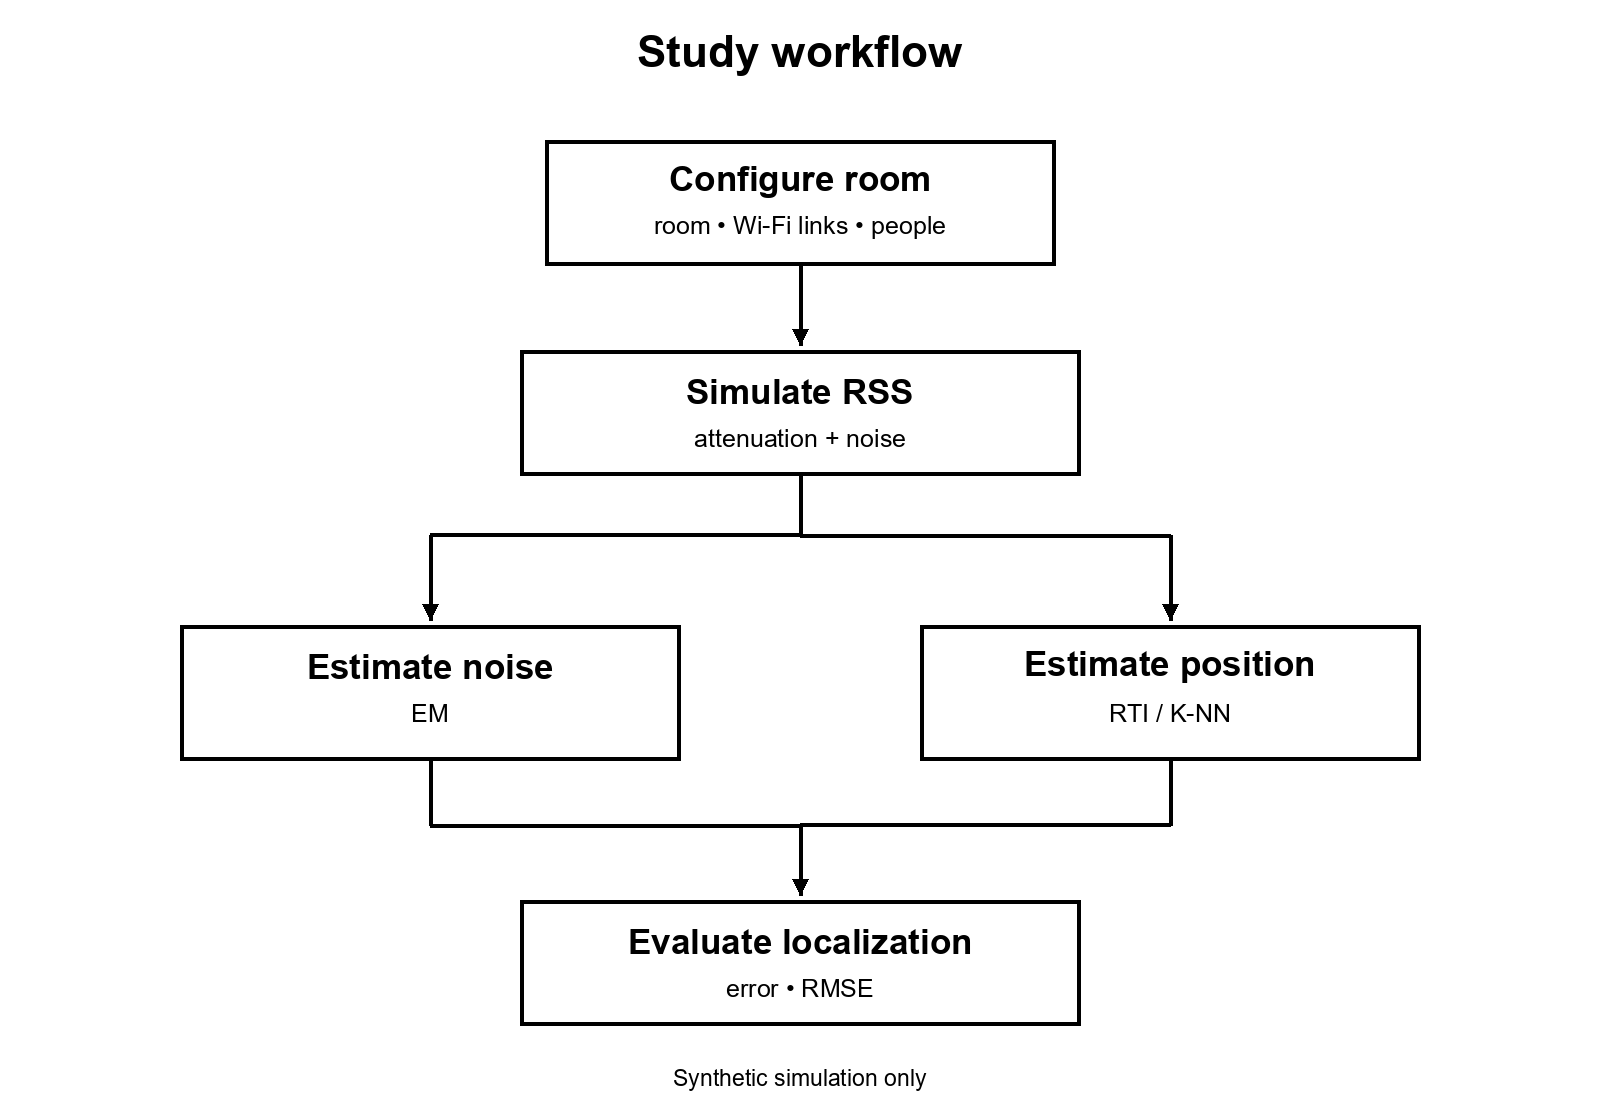
\includegraphics[width=10.5cm]{fig1.png}
\caption{Study workflow. The simulated room, links, and people are configured; RSS is simulated with attenuation and noise; EM estimates the noise model while RTI or K-NN estimates position; both feed the evaluation of localization error and RMSE. Synthetic simulation only.\label{fig:workflow}}
\end{figure}
\unskip

\subsection{Inputs, Partitions, and Algorithms}

The estimator receives calibration residuals after the reference estimate has been subtracted. The C++17 EM code estimates the mixture weight $p$ and both standard deviations while holding the component means at zero. A separate validation block compares the fitted mixture's average held-out log density with that of a single Gaussian. This measures how well each distribution predicts residuals; it does not measure localization accuracy.

The generator uses separate random streams for reference, calibration, noise validation, fingerprints, development, and test data. Development data selects regularization $\alpha$ and $K$; test data is reserved for scoring. K-NN fingerprints cover the same grid as the test locations but have independent noise draws. The current experiment therefore tests localization within a known grid. It does not test unseen positions, moving trajectories, multiple targets, or transfer to a different environment.

The localization comparison includes five methods: (1) Tikhonov RTI, (2) RTI with a Fisher factor calculated from the EM mixture, (3) a Tikhonov control with the equivalent regularization, (4) inverse-distance weighted K-NN on synthetic fingerprints, and (5) a constant prediction at the room center. In this implementation, the Fisher factor only rescales the Tikhonov penalty. The matched control checks that algebra; the equality does not demonstrate link-specific noise handling.

\subsection{Metrics and Planned Experiments}

For noise fit, the study records EM convergence, estimated parameters, and mean held-out log density (natural log per residual; residuals are in dB). For localization, it reports mean Euclidean error, RMSE in meters, and coverage. Mean, median, and RMS position error are the metrics reported by the RTI and RF-localization studies reviewed above \cite{Huang2020,Zhao2011,Kaltiokallio2021,Bahl2000}, and the held-out log density measures how well a fitted distribution predicts unseen residuals. The saved tables identify missing predictions and any center fallback. The current pilot uses one seed. The final evaluation will repeat the base and stress scenarios with independent seeds, summarize variation across runs, and compare methods on the same test queries.

The next stage will first reproduce the nine-scenario pilot, then repeat it across seeds to measure variability and convergence. The larger base geometry will also be run with several seeds. Correlated-noise and low-margin cases will be reported as failures or insufficient calibration whenever the estimator cannot fit the data. Each run saves its configuration, code hashes, generated CSVs, predictions, and summary. The main pipeline uses Python, NumPy, Matplotlib, and the existing C++17 EM code. Optional pandas and SciPy are only needed for diagnostics adapted from the upstream repository.

The planned schedule (Table~\ref{tab:schedule}) assumes four weeks, with a fifth week available if the final validation requires more time. During week 1, the existing pilot will be reproduced and its baselines fixed. During week 2, a position-likelihood estimator using the fitted Gaussian mixture will be implemented alongside a single-Gaussian control; attenuation will be estimated from development data. During week 3, both methods will be compared across independent seeds, node counts, measurement windows, off-grid positions, and correlated noise. During week 4, the analysis, code archive, and presentation will be finalized, and limitations or convergence failures will be reported. If a fifth week is available, a public RSS dataset may be explored as a separate external check, subject to compatible measurement metadata. Required resources are a standard Windows computer, Python with NumPy and Matplotlib, and a C++17 compiler. No Wi-Fi capture hardware is required for the synthetic study.

\begin{table}[H]
\caption{Planned work schedule.\label{tab:schedule}}
\begin{tabularx}{\textwidth}{>{\centering\arraybackslash}p{1.8cm}LL}
\toprule
\textbf{Week} & \textbf{Work} & \textbf{Deliverable}\\
\midrule
1 & Reproduce pilot; freeze metrics, data partitions, and baseline settings. & Reproduction record and evaluation protocol.\\
2 & Implement the mixture-based position likelihood and Gaussian control; estimate attenuation from development data. & Tested estimators and a documented development procedure.\\
3 & Compare independent seeds, node counts, measurement windows, off-grid positions, and correlated noise. & Comparative metrics, convergence records, and failure analysis.\\
4 & Finalize the proposal, reproducibility archive, results, and class presentation. & Complete submission package and presentation.\\
5 (optional) & Examine a compatible public RSS dataset as an external check. & Separate exploratory validation, if data format permits.\\
\bottomrule
\end{tabularx}
\end{table}

\subsection{Baselines and Validity Checks}

Tikhonov RTI is the main algorithmic baseline, following the foundational RTI formulation \cite{Wilson2010}. Its equivalent-regularization control checks whether the Fisher factor does anything beyond changing the penalty strength. Weighted K-NN provides a fingerprint comparison inspired by RF location systems \cite{Bahl2000}, and the room-center prediction checks whether the signal-based methods improve on a simple spatial prior. Calibration and validation data are disjoint. Hyperparameters are selected with development data and are fixed before test scoring.

The simulator also checks that CSV values survive a write-read cycle, link identities remain consistent, missing values stay marked, and each run records its parameter sources. Correlated noise violates the independence assumption of the base mixture model, and EM may fail to converge under that condition. When a low receiver margin leaves too few calibration residuals, the run stops before fitting. In either case, the summary reports the failure or insufficient calibration and omits a localization score when the pipeline cannot validly produce one.

\subsection{Reproducibility}

The project repository (\url{https://github.com/Camimilo-11/Ai-Yachay-2026/tree/main/Project-safe-wireless}) holds the simulator, the EM calibration code, the evaluation scripts, the run configurations with seeds and code hashes, the raw synthetic data, a requirements file, and the generated predictions, summaries, and figures. A verification script checks the package; one command (\texttt{ejecutar\_integracion.py -{}-quick -{}-suite}) runs the nine short scenarios, and a second command with the base configuration runs the full 12-node, 100-cell setup. Each run writes to a new output folder, and the README documents the steps. The required software is Python 3.10 or later and a C++17 compiler (g++); the Python scripts are the reproduction workflow, so no notebook is needed. All data are synthetic, so no external dataset is needed and no private or restricted data are published.

\section{Preliminary Results}

The quick base run used seed 7, six nodes, 15 links, 36 cells, and 30 test queries. EM converged after 294 iterations using 900 calibration residuals. It estimated $\hat{p}=0.541$, $\hat{\sigma}_1=1.060$~dB, and $\hat{\sigma}_2=2.938$~dB. For 450 held-out residuals, the mixture's mean log density was $-2.101$; the single Gaussian's was $-2.145$. The difference is small and comes from one generated split. Table~\ref{tab:results} reports the localization results.

\begin{table}[H]
\caption{Localization results of the quick base run (seed 7, 30 test queries).\label{tab:results}}
\begin{tabularx}{\textwidth}{>{\raggedright\arraybackslash}XCCC}
\toprule
\textbf{Method} & \textbf{Mean Localization Error (m)} & \textbf{RMSE (m)} & \textbf{Coverage}\\
\midrule
Tikhonov RTI & 3.653 & 4.113 & 30/30\\
EM-derived Fisher RTI & 3.530 & 4.015 & 30/30\\
Matched Tikhonov & 3.530 & 4.015 & 30/30\\
Weighted K-NN & 2.529 & 2.836 & 30/30\\
Constant room center & 2.357 & 2.517 & 30/30\\
\bottomrule
\end{tabularx}
\end{table}

The center prediction has the lowest mean error in this pilot, while K-NN performs better than either RTI setting. The Fisher-based RTI and its equivalent Tikhonov control agree to numerical precision, as expected from the equations. In the stress suite, EM did not converge within 600 iterations when temporal correlation was set to $\rho=0.8$. At 5~GHz with a low receiver margin, only 1.3\% of test measurements remained valid, so the run was marked insufficient for calibration. These outcomes come from simulated conditions, not a measured radio channel.

The files under \texttt{results/integracion\_verificada/} contain the reported values. The table uses \texttt{base\_r00/summary.json} and can be regenerated with the command in the README. This is an executed simulation with one seed; it is not a physical experiment.

\section{Discussion and Expected Research Direction}

The pilot shows that the mixture can be fitted and the RTI and fingerprint methods can run from generated CSV files. It also separates two different outcomes: the mixture has a slightly better held-out residual score, but none of the signal-based methods beats the room-center prediction in mean location error. The Fisher-based RTI offers no change beyond its effective regularization; the matched Tikhonov control produces the same result.

The next stage should repeat each scenario with several seeds and report variation in both residual scores and location errors. It should also measure parameter recovery, since the simulator's true mixture parameters are known, and check predictive fit under quantization, drift, missing links, and correlation. A future extension could estimate link-specific responsibilities together with the attenuation field, following the broader direction of noise-adaptive RTI \cite{Huang2020}. That would require a separate implementation and evaluation.

To move toward presence detection, a later simulation could add independent cases with and without an attenuation target, choose a decision threshold on development data, and measure sensitivity and false-alarm rate on held-out cases. This extension is not implemented in the current pilot, whose test queries all contain a target. It would still represent an idealized target without debris or material properties. Evaluating people under rubble would require a separate, subsequent study with suitable physical measurements, sensing geometry, and validation.

The pilot has several limits. Its base case uses synthetic independent noise; fingerprint and test locations share one grid; and each query contains one stationary target. The propagation model uses geometry rather than electromagnetic simulation, so reflections, diffraction, wall absorption, IEEE 802.11 MAC behavior, and CSI are outside its scope. Results from measured RSS and CSI studies provide context but do not predict this simulator's performance \cite{Wilson2010,Huang2020,Kaltiokallio2021}.

\section{Conclusions}

This study provides a reproducible comparison of mixture fitting and localization, with controls for regularization strength and a no-signal position prior. The pilot provides no evidence that EM improves position estimates. Conclusions will depend on repeated runs and apply only to the simulated conditions.

%=================================================================
\funding{This research received no external funding.}

\institutionalreview{Not applicable.}

\dataavailability{The generator, configuration, preliminary synthetic CSV files, predictions, summaries, and plotting outputs are included in the accompanying project repository: \url{https://github.com/Camimilo-11/Ai-Yachay-2026/tree/main/Project-safe-wireless}. No external dataset is required to reproduce the reported preliminary simulation. The README gives the execution commands, and each run records its configuration, seed, and code hashes.}

\useofartificialintelligence{Generative AI was used to assist with language editing, preparation of the LaTeX document, generation of the web page used to simulate and visualize the scenarios, and correction of the scripts. The simulation data and preliminary numerical results were produced by running the scripts, not generated by AI.}

\acknowledgments{This work was developed for the Artificial Intelligence course (instructor: Eugenio Morocho) and is linked to the Analysis of Algorithms course (instructor: Israel Pineda), both at Yachay Tech University.}

\conflictsofinterest{No conflicts of interest.}

%=================================================================
\begin{adjustwidth}{-\extralength}{0cm}

\reftitle{References}

\isAPAandChicago{}{%
\begin{thebibliography}{999}

\bibitem[Wilson and Patwari(2010)]{Wilson2010}
Wilson, J.; Patwari, N. Radio Tomographic Imaging with Wireless Networks. {\em IEEE Trans. Mob. Comput.} {\bf 2010}, {\em 9}, 621--632. \url{https://doi.org/10.1109/TMC.2009.174}.


\bibitem[Takeuchi et al.(2008)]{Takeuchi2008}
Takeuchi, T.; Saito, H.; Ohya, A.; Aoki, Y.; Matsuno, H.; Akiyama, I. Rescue Radar System with Array Antennas. {\em Trans. Soc. Instrum. Control Eng.} {\bf 2008}, {\em 44}, 962--969. \url{https://doi.org/10.9746/ve.sicetr1965.44.962}.


\bibitem[Gao et al.(2017)]{Gao2017}
Gao, F.; Sun, C.; Liu, H.; An, J.; Xu, S. An Image Restoration Method Using Matrix Transform and Gaussian Mixture Model for Radio Tomographic Imaging. {\em Wirel. Commun. Mob. Comput.} {\bf 2017}, {\em 2017}, 5703518. \url{https://doi.org/10.1155/2017/5703518}.


\bibitem[Huang and Yang(2020)]{Huang2020}
Huang, K.; Yang, Z. Noise Adaptive Optimization Scheme for Robust Radio Tomographic Imaging Based on Sparse Bayesian Learning. {\em IEEE Access} {\bf 2020}, {\em 8}, 118174--118182. \url{https://doi.org/10.1109/ACCESS.2020.3005048}.


\bibitem[Dempster et al.(1977)]{Dempster1977}
Dempster, A.P.; Laird, N.M.; Rubin, D.B. Maximum Likelihood from Incomplete Data via the EM Algorithm. {\em J. R. Stat. Soc. Ser. B Methodol.} {\bf 1977}, {\em 39}, 1--22. \url{https://doi.org/10.1111/j.2517-6161.1977.tb01600.x}.


\bibitem[Wu(1983)]{Wu1983}
Wu, C.F.J. On the Convergence Properties of the EM Algorithm. {\em Ann. Stat.} {\bf 1983}, {\em 11}, 95--103. \url{https://doi.org/10.1214/aos/1176346060}.


\bibitem[Zhao and Patwari(2011)]{Zhao2011}
Zhao, Y.; Patwari, N. Robust Estimators for Variance-Based Device-Free Localization and Tracking. {\em arXiv} {\bf 2011}, arXiv:1110.1569. \url{https://arxiv.org/abs/1110.1569}.


\bibitem[Kaltiokallio et al.(2021)]{Kaltiokallio2021}
Kaltiokallio, O.; Hostettler, R.; Y\u{i}\u{g}itler, H.; Valkama, M. Unsupervised Learning in RSS-Based DFLT Using an EM Algorithm. {\em Sensors} {\bf 2021}, {\em 21}, 5549. \url{https://doi.org/10.3390/s21165549}.


\bibitem[Bahl and Padmanabhan(2000)]{Bahl2000}
Bahl, P.; Padmanabhan, V.N. RADAR: An In-Building RF-Based User Location and Tracking System. In Proceedings of the IEEE INFOCOM 2000, Tel Aviv, Israel, 26--30 March 2000; Volume~2, pp. 775--784. \url{https://doi.org/10.1109/INFCOM.2000.832252}.


\bibitem[IsukaW()]{IsukaW}
IsukaW. wifi-sensing-human-presence. GitHub repository, revision 91aee04ea938274d014a3981d409f83267ea15c0. Available online: \url{https://github.com/IsukaW/wifi-sensing-human-presence/tree/91aee04ea938274d014a3981d409f83267ea15c0} (accessed on 27 October 2026).

\end{thebibliography}
}

\end{adjustwidth}
\end{document}
